%
% injektiv.tex
%
% (c) 2021 Prof Dr Andreas Müller, OST Ostschweizer Fachhochschule
%
\bgroup
\def\sx{1.05}
\begin{frame}[t]
\frametitle{$f$ injektiv auf $\mathcal{J}(f)$}
\setlength{\abovedisplayskip}{8pt}
\setlength{\belowdisplayskip}{8pt}
\vspace{-15pt}
\begin{columns}[t,onlytextwidth]
\begin{column}{0.58\textwidth}
\begin{center}
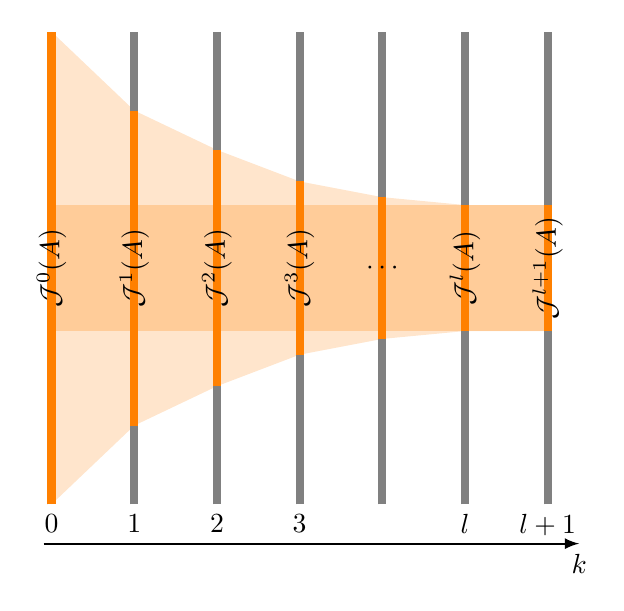
\begin{tikzpicture}[>=latex,thick]

\fill[color=orange!20]
	({0*\sx},-3.0) -- ({1*\sx},-2.0) -- ({2*\sx},-1.5) --
	({3*\sx},-1.1) -- ({4*\sx},-0.9) -- ({5*\sx},-0.8) --
	({6*\sx},-0.8) --
	({6*\sx},0.8) -- ({5*\sx},0.8) -- ({4*\sx},0.9) --
	({3*\sx},1.1) -- ({2*\sx},1.5) -- ({1*\sx},2.0) --
	({0*\sx},3.0) -- cycle;
\fill[color=orange!40] (0,-0.8) rectangle ({6*\sx},0.8);

\foreach \x in {0,...,6}{
	\draw[color=gray,line width=3pt] ({\x*\sx},-3)--({\sx*\x},3);
}
\foreach \x in {0,1,2,3}{
	\node at ({\sx*\x},-3) [below] {$\x$};
}
\node at ({\sx*5},-3) [below] {$l$};
\node at ({\sx*6},-3) [below] {$l+1$};
\draw[->] (-0.1,-3.5) -- ({6*\sx+0.4},-3.5) coordinate[label={below:$k$}];

\draw[line width=3pt,color=orange] ({0*\sx},-3.0) -- ({0*\sx},3.0);
\draw[line width=3pt,color=orange] ({1*\sx},-2.0) -- ({1*\sx},2.0);
\draw[line width=3pt,color=orange] ({2*\sx},-1.5) -- ({2*\sx},1.5);
\draw[line width=3pt,color=orange] ({3*\sx},-1.1) -- ({3*\sx},1.1);
\draw[line width=3pt,color=orange] ({4*\sx},-0.9) -- ({4*\sx},0.9);
\draw[line width=3pt,color=orange] ({5*\sx},-0.8) -- ({5*\sx},0.8);
\draw[line width=3pt,color=orange] ({6*\sx},-0.8) -- ({6*\sx},0.8);

\foreach \x in {0,1,2,3}{
	\node at ({\x*\sx},0) [rotate=90] {$\mathcal{J}^{\x}(A)$};
}
\node at ({4*\sx},0) {$\cdots$};
\node at ({5*\sx},0) [rotate=90] {$\mathcal{J}^{l}(A)$};
\node at ({6*\sx},0) [rotate=90] {$\mathcal{J}^{l+1}(A)$};

\end{tikzpicture}
\end{center}
\end{column}
\begin{column}{0.38\textwidth}
\begin{block}{stationär}
$l$ der $k$-Wert, ab dem gilt
\begin{align*}
\mathcal{J}^l(A) &= \mathcal{J}^{l+1}(A) = A\mathcal{J}^l(A)
\end{align*}
\end{block}
\vspace{-10pt}
\uncover<2->{%
\begin{block}{Dimension}
\vspace{-10pt}
\[
\dim \mathcal{J}^l(A) = \dim\mathcal{J}^{l+1}(A)
\]
\uncover<3->{%
d.~h.~$A$ ist bijektiv als Selbstabbildung von
$\mathcal{J}(A)$}
\uncover<4->{%
\[
\Downarrow
\]
$A|\mathcal{J}(A)$ ist injektiv}
\end{block}}
\end{column}
\end{columns}
\end{frame}
\egroup
